\documentclass{article}
\usepackage[a4paper, total={5in, 8in}]{geometry}
\usepackage{hyperref}
\usepackage{amsmath}
\usepackage{graphicx}
\usepackage[utf8]{inputenc}
\usepackage[T1]{fontenc}
\usepackage[spanish]{babel}
\usepackage{mdframed}

\selectlanguage{spanish}
\graphicspath{ {figs/} }

\newmdenv[leftline=false,rightline=false]{topbot}
\newtheorem{pregunta}{Pregunta}

\font\domino=domino
\def\die#1{{\domino#1}}

\DeclareFontFamily{U}{skulls}{}
\DeclareFontShape{U}{skulls}{m}{n}{ <-> skull }{}
\newcommand{\skull}{\text{\usefont{U}{skulls}{m}{n}\symbol{'101}}}

\begin{document}
\begin{center}
  \Large Parcial 1 \\
  %\die1 \die2 \die3 $\skull$ \die4 \die5 \die6 \\
  Estadística.
\end{center}
\vspace{1cm}
\begin{tabular}[t]{c}
  \textbf{Paralelo B} \\ [10pt]
  \textbf{Nombre: \rule{4cm}{0.15mm}} \\
  \\
  \textbf{Fecha: \rule{4cm}{0.15mm}}
\end{tabular}
\null\hfill
\begin{tabular}[t]{c c}
  P. 1: & \quad \rule{0.5cm}{0.15mm}/4\\[6pt]
  P. 2: & \quad \rule{0.5cm}{0.15mm}/4\\[6pt]
  P. 3: & \quad \rule{0.5cm}{0.15mm}/4\\[6pt]
  P. 4: & \quad \rule{0.5cm}{0.15mm}/4\\[6pt]
  P. 5: & \quad \rule{0.5cm}{0.15mm}/4\\[6pt]
  Nota: & \quad \rule{0.5cm}{0.15mm}/20
\end{tabular}

\null\hfill

\textbf{Importante:\\
 Escriban el código R para TODAS las preguntas de programación. \\ Es un trabajo INDIVIDUAL.}
 \begin{topbot}
   \vspace{0.7em}
   Ejercicio 1 \quad Lectores, notas y Libros
   \vspace{0.7em}
 \end{topbot}

Para este ejercicio van a necesitar dos tablas: libros y notas\_lector. La tabla libros contiene una lista de libros. En notas\_lector van a encontrar una lista de usuarios que calificaron algunos de los libros.
\begin{pregunta} (4 puntos)
Escriban el c\'odigo para saber cuales son los lectores que leyeron la mayor cantidad de libros.
\end{pregunta}
\framebox(360,130){} \\
\par
\begin{pregunta} (4 puntos)
Escriban el código para crear una tabla con las notas promedio por libro. Unan esa tabla con libros. Cuál es el libro que tiene la peor nota en promedio?
\end{pregunta}
\framebox(350,130){} \\

\begin{topbot}
  \vspace{0.7em}
  Ejercicio 2 \quad Nacimientos y viernes 13
  \vspace{0.7em}
\end{topbot}

Para este ejercicio van a necesitar la tabla nacimientos. La tabla contiene el número de nacimientos en Estados Unidos de Norte América por día entre los años 2000 y 2014.
\begin{pregunta} (4 puntos)
Escriban el código que produce una tabla con el número de nacimientos en el 2009 por día. Cuántos días fueron vierens 13 ese año?
\end{pregunta}
\framebox(360,130){} \\
\par
\begin{pregunta} (4 puntos)
Qué hacen estas líneas de código?
\begin{align*}
  ggplot(nacimientos,\ & aes(x=dia\_semana, \ y=nacimientos)) \ + \\
    & \ geom\_bar(stat='identity')
\end{align*}

\end{pregunta}
\framebox(350,130){} \\

\begin{pregunta} (4 puntos)
La figura \ref{fig:hist} contiene el histograma del número de viernes 13 por año. Cuántos viernes 13 hay en total? Cuántos viernes 13 hay en promedio en un año? Cuál es la proporción de viernes 13 entre el 2000 y el 2007?
\end{pregunta}
\framebox(350,100){}
\begin{figure}[ht]
  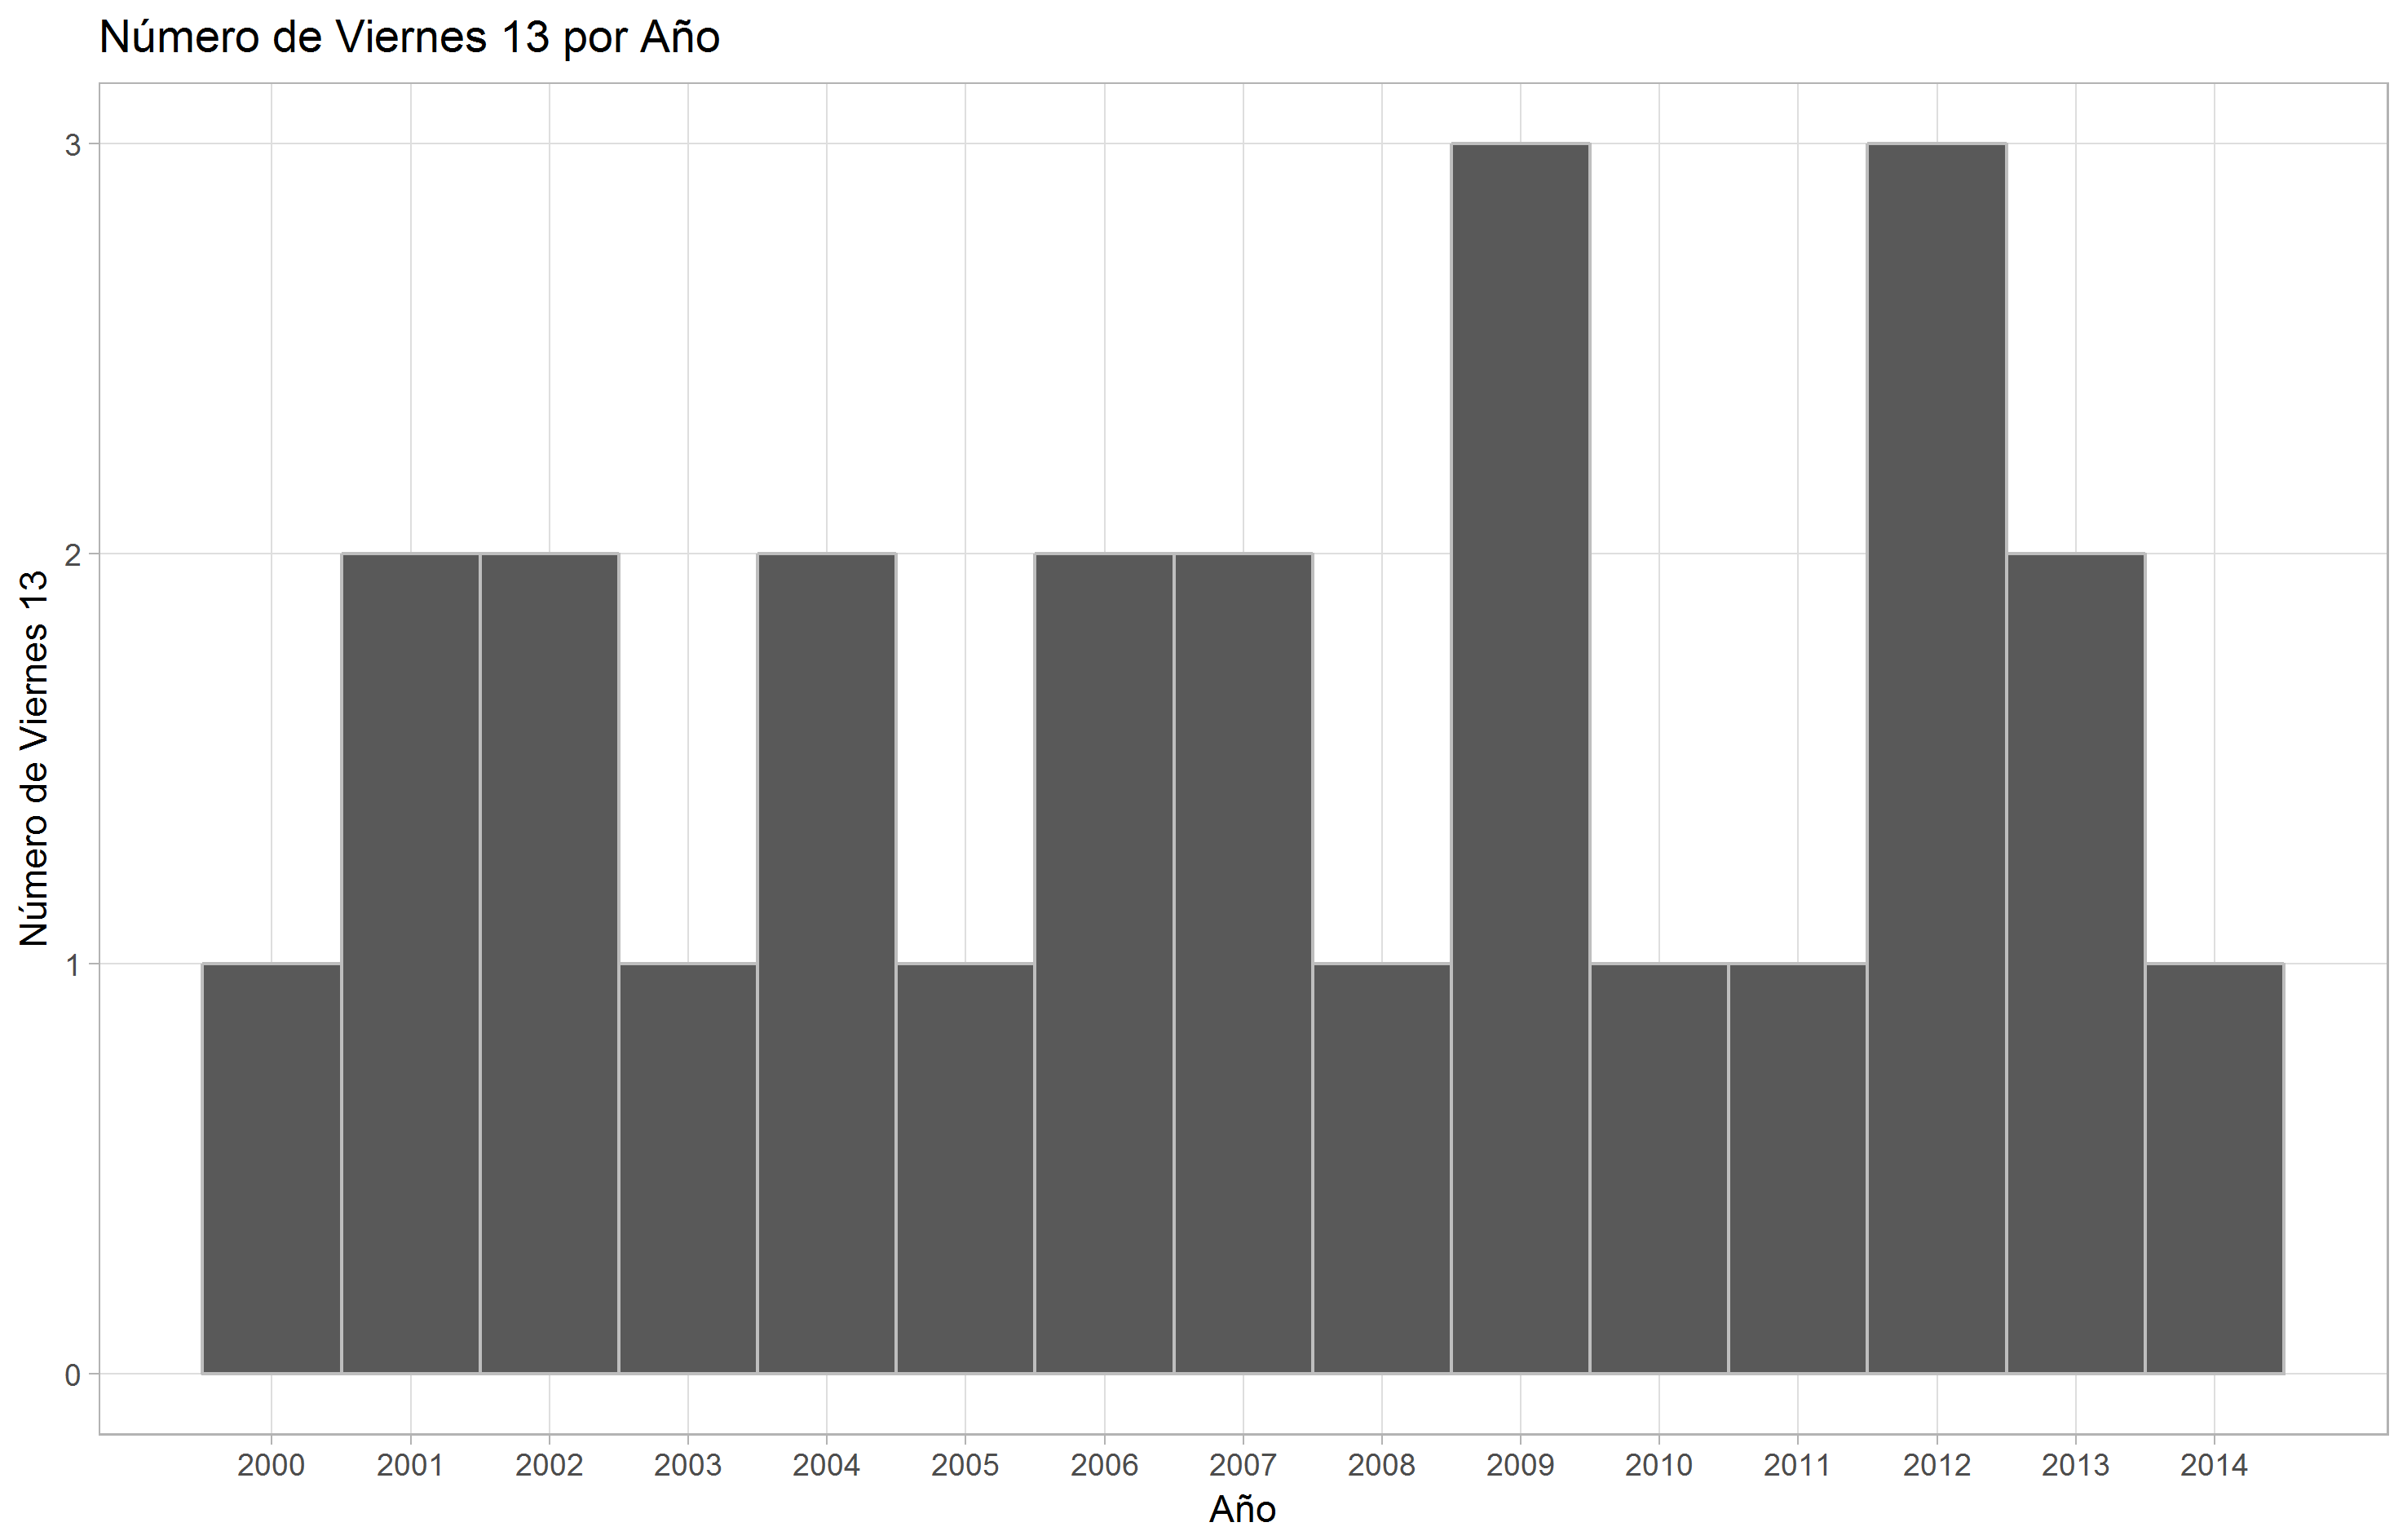
\includegraphics[scale = 0.45] {Viernes13.png}
  \caption{Histograma pregunta 5. }
  \label{fig:hist}
\end{figure}
\end{document}
